\large

\section{Hadronically decaying $\tau$ lepton}
\label{sec:rec:tau}
With a mass of 1.777 GeV and a proper decay length
of 87 $\mu$m~\cite{PDG}, tau leptons decay either leptonically
($\tau_{lep} \rightarrow \ell \nu \ell \nu \tau$, $\ell  = e, \mu$ ) 
or hadronically ($\tau_{had} \rightarrow$ hadrons $\nu_{\tau}$) 
and do so typically before reaching active
regions of the \hbox{ATLAS} detector. 
The leptonically decaying $\tau_{lep}$ is simply reconstructed
as either an electron or muon, with the netrinos contributing 
to the real component of the \met. 
On the other hand, the hadronically decaying $\tau_{tau}$ 
can be identified via their decay products. 
The hadronic tau lepton decays represent 65\% of all possible decay modes~\cite{PDG}. 
In these decay modes, the hadronic decay products are 
one or three charged pions in 72\% and 22\% of all cases, respectively. 
Charged kaons are present in the 
majority of the remaining hadronic decays. 
In 78\% of all hadronic decays, up to one associated neutral pion is
also produced. The neutral and charged hadrons stemming from 
the tau lepton decay make up the visible
decay products of the tau lepton, 
and are in the following referred to as $\tau_{had-vis}$.
\subsection{Reconstruction}
The $\tau_{had-vis}$ candidates are
seeded by jets formed using the anti-$k_t$ algorithm,
with a jet-size parameter $R$ of 0.4. 
For events with multiple interactions, the chosen primary may not be the
vertex where the tau lepton is originated. 
There the \textit{tau vertex association} algorithm is used with 
input as all tau candidates tracks within a region of $\Delta R$ < 0.2 
around the jet seed direction. 
The \pt\ of these tracks is summed and the 
primary vertex candidate to which the largest fraction
of the \pt\ sum is matched to is chosen as the tau vertex~\cite{ATLAS-CONF-2014-018}.

Tracks are associated with the $\tau_{had-vis}$ if they are
in the \textit{core} region $\Delta R$ < 0.2 
around the $\tau_{had-vis}$ direction and 
satisfy the following criteria: \pt\ > 1 GeV, 
at least two associated hits in the pixel layers of the inner detector, 
and at least seven hits in total in the pixel and the SCT layers. 
Furthermore, requirements are imposed on 
the distance of closest approach of the track to the track vertex
in the transverse plane, $|d_0|$ < 1.0 mm, and
longitudinally, $|z_0 sin\theta|$ < 1.5 mm. 
Tracks in the \textit{isolation} region 0.2 < $\Delta R$ < 0.4 
are used for the calculation of identification variables 
and are required to satisfy the same selection criteria.
% A set of boosted decision trees (BDTs) is used to classify all 
% tracks within $\Delta R$ = 0.4 of the $\tau_{had-vis}$ axis 
% into core and isolation tracks, depending on their \pt, 
% the number of hits in the tracking detectors 
% as well as their transverse and
% longitudinal impact parameters with respect to the tau vertex. 
The number of core tracks defines the number of \textit{prongs}.

\subsection{Identification}
The $\tau_{had-vis}$ reconstruction algorithm alone provides 
no discrimination against other particles that result in
jet-like signatures in the detector. 
Therefore, dedicated algorithms are used to identify hadronic tau lepton
decays. Here, a recurrent neural network (RNN) classifier 
is used as described in reference~\cite{ATL-PHYS-PUB-2019-033}.
Compared to the ID that was used in the analysis of the 36.1 fb$^{-1}$ data~\cite{HIGG-2016-16},
which was based on a boosted decision tree, 
the RNN tau-ID shows better performance 
and allows to move to a looser WP gaining increased efficiency 
(about 24\% and 11\% in case of two $\tau_{had}$ and 
one $\tau_{had}$ in the final state, respectively) 
without losing jet rejection, as shown in Figure~\ref{fig:RNNtau}. 
Due to the distinct signatures of 1- and 3-prong $\tau_{had}$ decays, 
the $\tau_{had}$--identification ($\tau_{had}$--ID) is split into dedicated
algorithms for 1- and 3-track $\tau_{had-vis}$.
Selected $\tau_{had-vis}$ candidates in the analysis are required to have 
\pt\ > 20 GeV, $|\eta|$ < 2.5, with candidates in the barrel-endcap 
transition region of the calorimeter (1.37 < $|\eta|$ < 1.52) vetoed 
due to poor detector instrumentation in this region, 
one or three tracks, unit charge, and to pass the ‘loose’ $\tau_{had}$--ID working point.
The loose WP corresponds to 85\% efficiency for 1-prong 
and 75\% efficiency for 3-prong (the efficiency is
flat in \pt\ by definition).
\begin{figure}[bth]
	\begin{centering}	
	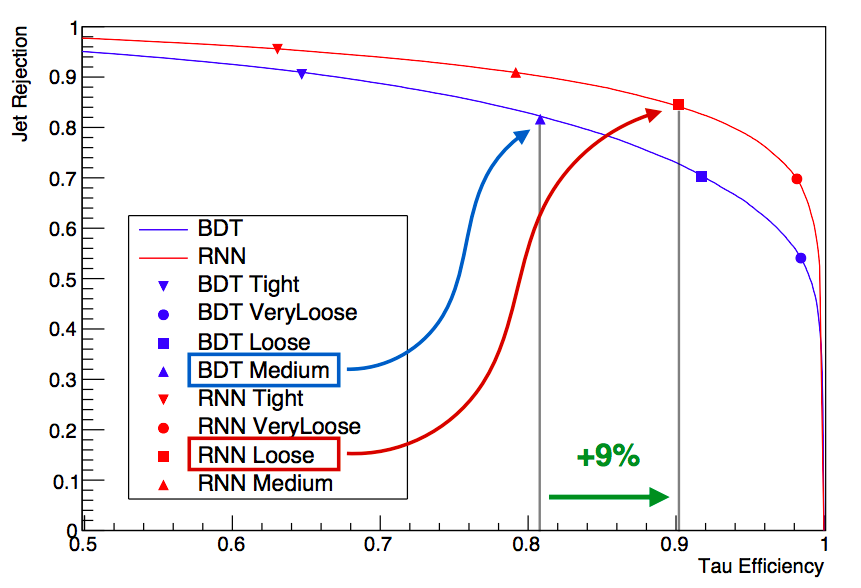
\includegraphics[width=.9\textwidth]{Reconstruction/plots/tauRNN.png}
	\caption{Jet rejection and tau efficiency of tau candidate, 
    measured in $\gamma^* \rightarrow \tau\tau$ sample for RNN-ID~\cite{ATL-PHYS-PUB-2019-033}
    and $Z/\gamma^* \rightarrow \tau\tau$ sample for BDT-ID~\cite{ATL-PHYS-PUB-2015-045}.
    Jet rejection represents the probability of a jet 
    not originating from a tau lepton being rejected 
    by the identification algorithm.
    The green arrow indicates the increase in tau efficiency.}
	\label{fig:RNNtau}
	\end{centering}
\end{figure}

Additional rejection of $\tau_{had-vis}$ candidates originating 
from electrons is provided by a BDT employing track
and shower shape information, the `loose' working point is used, 
corresponding to a selection efficiency
of about 95\% efficiency for true $\tau_{had-vis}$~\cite{ATLAS-CONF-2017-029}.
% Studies on the comparison between the BDT 
% (used in the previous round of the analysis) and RNN $\tau_{had}$--IDs
% and on the choice of the working point are reported in Appendix C.3. 

\subsection{Anti--$\tau_{had}$ definition}
In order to provide fake--$\tau_{had}$--enriched regions used for background estimation, 
an ``anti--$\tau_{had}$'' selection is defined. 
Those $\tau_{had-vis}$ objects that fail the RNN loose $\tau_{had}$--ID 
and have the RNN score greater than 0.01 are labelled as anti--$\tau_{had}$ candidates. 
For channels where $\tau_{had}$--ID is applied at trigger level, anti--$\tau_{had}$
candidates are also required to be matched to the trigger $\tau_{had}$ in 
the same way as is required for signal taus.
This definition selects objects that are 
predominantly jets faking hadronic $\tau$ decays. 
The minimum RNN score requirement ensures that 
the jets still have some $\tau_{had}$-like properties 
and ensures that the composition of quark- and gluon-initiated jets 
is closer to that of the signal region.
More details of the choice of the minimum $\tau_{had}$--ID RNN-score
threshold are reported in TODO: link to the fake factor section
% RNN score < 0.01 is chosen as it is the cut used and recommended by the Fake-Tau-Task-Force and was
% also tested here to give an improvement in the statistical precision of the multi-jet fake-factors and of the
% multi-jet template compared to the "VeryLoose" working point (RNN score < 0.05, with 95\% efficiency
% for true-$\tau_{had}$).
% Internal note C.4.1:
% The RNN > 0.01 is used by the Fake-Tau-Task-Force and has been studied here to extend the anti-tauhad
% 2526 control regions and check the impact of the reduced statistical uncertainties on the FFs and of the reduced
% 2527 statistical uncertainties on the multi-jet template.
% 2528 Lowering the cut from RNN > 0.05 of the VeryLoose to RNN > 0.01 gives an improvement in the
% 2529 statistical precision of the FFs (about 10-15% reduction in relative uncertainty) which translates in smaller
% 2530 systematic uncertainties from this source on the multi-jet template and more importantly it reduces the
% 2531 statistical uncertainty on the multi-jet tempalte itsfelf by reduced by approximately 30% given the increased
% 2532 statistics in the Anti-ID OS region where the FFs are applied to obtain the template for the SR, as shown in
% 2533 Figure 166.
\subsubsection{Anti--$\tau_{had}$ selection: TODO: should I put this section in here or in analysis chapter?}
Anti--$\tau_{had}$ objects are selected only in events 
in which there are fewer $\tau_{had}$ that pass the offline $\tau_{had}$--ID than
required for a given channel (one for the $\tau_{lep}\tau_{had}$ 
and two for the $\tau_{had}$$\tau_{had}$ selection). 
In that case, additional anti--$\tau_{had}$ candidates are selected 
so that the total number of selected $\tau_{had}$ (loose, which always has priority,
and anti--$\tau_{had}$) corresponds to the required multiplicity in each channel.
For channels where $\tau_{had}$--ID is applied at trigger level 
(more details in Section~\ref{sec:event selection}), 
only the anti--$\tau_{had}$ objects that are matched to the
trigger $\tau_{had}$ are considered, and thus there are 
no multiple selection possibilities. 
However, for channels where a $\tau_{had}$ trigger is not used, 
an anti--$\tau_{had}$ candidate is chosen randomly when there are more reconstructed
$\tau_{had}$ satisfying the anti--$\tau_{had}$ definition. 
Any anti--$\tau_{had}$ objects that are not selected in this process are also not
considered when performing the overlap removal of detector objects, 
which is discussed in Section~\ref{sec:overlap}.

\section{Missing transverse energy}
As defined in Equation~\ref{eq:MET}, the $\vec{E_T}^{miss}$ is defined 
as the negative vector sum of transverse momentum collected from the 
detector, from which one or more ``invisible'' particle(s) can be inferred. 
The reconstruction of $\vec{E_T}^{miss}$ is comprised of two contributions~\cite{MET2018}. 
The first one is from \textit{hard-event} signals combining 
information of fully reconstructed and calibrated 
physics objects, i.e. electrons, muons, photons, jets,
hadronically decaying $\tau$-leptons and jets. 
The second one is from the \textit{soft-event}, consisting of 
reconstructed charged-particle tracks associated with the hard-scatter
vertex but with no physics objects.

\section{Overlap removal}
After the event is reconstructed, an overlap-removal procedure is applied 
to resolve ambiguities when a physical object is reconstructed as multiple 
particles in the \hbox{ATLAS} detector. The angular distance $\Delta R$ is used 
to measure the overlap of two reconstructed objects.
Overlaps between most of the detector objects used in the analysis are resolved 
by using the standard overlap removal tools AssociationUtils~\cite{ORTool}, 
with analysis specific procedure for 
the reconstructed $\tau_{had-vis}$, anti-$\tau_{had-vis}$ objects and jets.
The step-by-step procedure that is used to resolve ambiguities in the 
reconstructed objects is summarised in  the following:
 \begin{itemize}
     \item  $e_1$--$e_2$: For two electrons $e_1$ and $e_2$ in an event,  
     reject $e_1$ if both electrons share the track and $p_{T1}$ < $p_{T2}$
    \item  $\tau_{had-vis}$--$e$: Reject $\tau_{had-vis}$ if $\Delta R$ < 0.2 
    % and   $e$ passes \hbox{DFCommonElectronsLHLoose}
    \item  $\tau_{had-vis}$--$\mu$: Reject $\tau_{had-vis}$ if $\Delta R$ < 0.2:
     \\ Case 1 ($\tau_{had-vis}$ $p_T$ > 50GeV): $p_T$, $\mu$ > 2GeV and combined muon
     \\ Case 2 ($\tau_{had-vis}$ $p_T$ $\leq$ 50GeV): $p_T$, $\mu$ > 2GeV
    \item  $\mu$--$e$: Reject $\mu$ if calo-muon and shared ID track
    \item  $e$--$\mu$: Reject $e$ if shared ID track
    \item  jet--$e$: Reject jet if $\Delta R$ < 0.2
    \item  $e$--jet: Reject $e$ if $\Delta R$ < 0.4
    \item  jet--$\mu$: Reject jet if $N_{track}$ < 3 ($p_{T}^{track}$ > 500MeV), and $\Delta R$ < 0.2
    \item  $\mu$--jet: Reject $\mu$ if $\Delta R$ < 0.4
 \end{itemize}
 Additionally, an analysis-specific overlap-removal procedure for $\tau_{had-vis}$, 
 anti-$\tau_{had-vis}$ and jets is implemented:
\begin{itemize}
    \item jet--$\tau_{had-vis}$: Reject jet if $\Delta R$ < 0.2
    \item anti--$\tau_{had-vis}$--jet: Reject anti--$\tau_{had}$ if jet is $b$-tagged and $\Delta R$ < 0.2
    \item jet--anti--$\tau_{had-vis}$: Reject jet if $\Delta R$ < 0.2
\end{itemize}
 This establishes the following priority: $\tau_{had-vis}$ > $b$-tagged jet > anti-$\tau_{had-vis}$ > un-tagged jet.
%  Another priority, $b$-tagged jet > $\tau_{had-vis}$ > anti-$\tau_{had-vis}$ > un-tagged jet, was investigated as an alternative
%  but found to reduce signal acceptance in the 2-tag region significantly due to limited $\tau_{had}$ rejection of the
%  DL1r $b$-tagging algorithm at the 77\% working point. With the alternative priority the signal acceptance is
%  reduced by about 8\% (13\%) in $\tau_{lep}$$\tau_{had}$ ($\tau_{had}$$\tau_{had}$).
\label{sec:overlap}

